\chapter{Inne algorytmy}

W poprzednim rozdziale skupiliśmy się głównie na algorytmie Dijkstry i~jego różnych implementacjach, wprowadzając też po drodze algorytmy, które stanowiły dla nas tło do dalszych rozważań (algorytm sortowania topologicznego, czy Bellmana-Forda). Rozpoczęliśmy od algorytmów o~kwadratowej złożoności obliczeniowej ($O \left( n^{2} \right)$), kończąc na implementacji kopców pozycyjnych, dla których czas działania w~najgorszym przypadku wynosił $O \left( m + n \cdot \log \left( C \right) \right) $. W~tym rozdziale będziemy chcieli zaprezentować kilka mniej znanych algorytmów, rozwiązujących problem najkrótszych ścieżek --- między innymi algorytmy zaproponowane przez U.Pape'a (algorytm $PAP$) oraz Stefana Pallottino (modyfikacja poprzedniego algorytmu)~\cite[$4.$]{GIDA}. Na końcu przedstawimy algorytm progowy, który jest algorytmem typu \textit{Label-Correcting}.

\section{Kombinacje struktur}

Do konstrukcji pierwszych dwóch algorytmów wykorzystamy połączenia dwóch różnych typów abstrakcyjnych struktur danych, którymi będą kolejki: $FIFO$ (ang. \textit{First In First Out}) oraz $LIFO$ (ang. \textit{Last In First Out}). Do implementacji pierwszej z~nich oryginalnie był wykorzystany stos, zaś drugą będziemy reprezentować przez zwykłą listę podwójnie dowiązaną.

\subsection{Algorytm przyrostowy}

Pseudokod algorytmu przyrostowego (ang. \textit{Graph Growth Algorithm}) wygląda identycznie jak ten, który przedstawiliśmy dla generycznego algorytmu Dijkstry. Różnica między tymi dwoma implementacjami wynika ze specyficznej struktury, jaka została zastosowana w~tym przypadku, a~której przykład znajduje się poniżej:


\begin{figure}[!htbp]
	\centering
	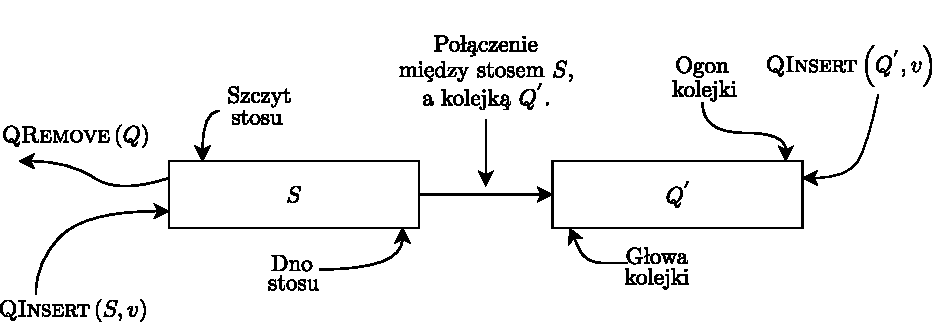
\includegraphics[width=\textwidth]{Chapter_III/GRAPH-GROWTH-1Q-Other/a.pdf}
	\caption{\textbf{Struktura wykorzystywana w~algorytmie $PAP$}} \label{fig:examplePAPStructure}
\end{figure}

W zastosowanym rozwiązaniu wyróżniamy dwie struktury, z~których pierwsza jest implementacją kolejki $FIFO$ (stos), druga zaś to zwykła kolejka typu $LIFO$. Obie są połączone ze sobą, co oznacza, że za ostatnim elementem, należącym do stosu $S$, znajduje się pierwszy wierzchołek w~kolejce $Q^{'}$. Dla takiej struktury wyróżniamy następujące operacje:

\begin{itemize}
\item $\textrm{\textsc{QRemove}} \left( S \right) $ --- usuwa ze szczytu stosu (lub początku kolejki $Q^{'}$, gdy stos jest pusty) wierzchołek $v$,
\item $\textrm{\textsc{QInsert}} \left( ?, v \right)$ --- gdy wierzchołka $v$ nie ma jeszcze ani na stosie $S$, ani w~kolejce $Q^{'}$, w~zależności od właściwości danego wierzchołka wykonujemy jedną z~możliwych operacji:
\begin{itemize}
\item $\textrm{\textsc{QInsert}} \left( S, v \right) $ --- jeżeli wierzchołek, w~momencie wstawiania, jest osiągalny ze źródła ($v.d < \infty$) to jest on wstawiany na szczyt stosu $S$,
\item $\textrm{\textsc{QInsert}} \left( Q, v \right) $ --- w~przeciwnym przypadku (gdy węzeł jest nieosiągalny --- $v.d = \infty$) wierzchołek wstawiany jest na koniec kolejki $Q^{'}$,
\end{itemize}
\end{itemize}

oraz, typową dla takiej struktury, operację $\textrm{\textsc{IS-EMPTY}} \left( Q \right) $, gdzie poprzez $Q$ oznaczymy całą, powyżej opisaną strukturę (jest ona pusta, gdy zarówno w~$S$ jak i~$Q^{'}$ nie ma wierzchołków). Dodatkowo chcemy, by pierwsza ze struktur (ta, z~której ściągamy elementy) miała własności kolejki priorytetowej~\cite[$4.$,$77$--$78$]{GIDA}.

\subsubsection{Uwagi do algorytmu}

Aby efektywnie zaimplementować kolejkę priorytetową, wykorzystując do tego stos, będziemy potrzebować albo rekurencyjnie wyciągać elementy ze stosu, aż do momentu, gdy natrafimy na odpowiednie miejsce, w~które włożymy nowy (bądź aktualizowany) element, albo możemy wykorzystać do tego drugi stos, przemieszczając elementy pierwszego stosu na drugi, porównując przy okazji każdy taki element z~tym, który chcemy na stos wstawić (niech będzie to element $v$). W~momencie, gdy z~pierwszego stosu wyciągniemy taki element $u$, dla którego $u.v \geqslant v.d$, wstawiamy na stos wierzchołek $v$ a~następnie z~powrotem przekładamy elementy z~pomocniczego stosu na ten właściwy. Pierwotna kolejność pozostałych elementów nie ulega zmianie. W~przypadku modyfikacji wierzchołka $v$ już będącego na stosie przekładamy elementy ze stosu do momentu, w~którym nie wyciągniemy interesującego nas węzła. Następnie przekładamy z~powrotem elementy, które dopiero co włożyliśmy na drugi stos, do momentu, w~którym na szczycie tego stosu nie znajdzie się wierzchołek $u$, którego $u.d \leqslant v.d$ (lub $u.d < v.d$~--- w~zależności co chcemy osiągnąć). Po wystąpieniu takiej sytuacji na oryginalny stos wstawiamy zaktualizowany element a~następnie kontynuujemy przerzucanie wierzchołków z~tymczasowego stosu, dopóki ten nie zostanie pusty a~na szczycie tego pierwszego z~powrotem nie znajdzie się element, który był tam uprzednio (chyba, że zaktualizowany element okaże się być teraz najmniejszym elementem na stosie). Należy jednak zwrócić uwagę, że w~oryginalnej implementacji nie mamy wsparcia dla operacji aktualizacji wierzchołka w~kolejce, więc własność kolejki priorytetowej dla stosu będziemy musieli całkowicie odbudowywać przy operacji $\textrm{\textsc{QRemove}} \left( S \right) $, zaś złożoność obliczeniowa w~najgorszym przypadku staje się wykładnicza.

\subsubsection{Złożoność obliczeniowa}

Jak w~każdym przypadku, gdzie wykorzystywaliśmy kolejki priorytetowe do zwracania wierzchołków $v$, takich że $v.d = \min \left\{ u \in Q \right\}$, także tutaj nasza analiza czasu działania algorytmu opierać się będzie na analizie kosztów, związanych z~kosztami wykonywania operacji na takiej kolejce (wzór \ref{eq:dijkstraComplexityShort}), a~zatem:

\begin{itemize}
\item w~każdym kroku algorytm trwale usuwa jeden wierzchołek $v$ z~kolejki, którego $v.d = \delta \left( s, v \right)$ (jak udowodniliśmy w~\ref{pr:dijkstra}).
\item Wyszukanie na stosie takiego elementu $v$, by $v.d = \min \left\{ u \in Q \right\}$ w~najgorszym przypadku zajmie $ O \left( n \right) $ (gdzie przy wykorzystaniu dwóch stosów sprowadzi się to do wyciągnięcia wszystkich elementów z~pierwszego, zapamiętania najmniejszego podczas wstawiania ich na drugi stos, a~następnie --- przy operacji odwrotnej --- wstawić na pierwszy stos, wyciągając kolejno elementy ze stosu tymczasowego, wszystkie wierzchołki, poza tym najmniejszym).
\item Algorytm wykona skanowanie każdego wierzchołka dokładnie jeden raz, więc liczba relaksacji, jakie wykona, będzie równa $m$.
\end{itemize}

Da nam to złożoność algorytmu $PAP$ na poziomie $ O \left( m + n^{2} \right)$.\footnote{Jeżeli zrezygnowalibyśmy z wyszukania minimalnych elementów na stosie to złożoność czasowa może sięgać nawet czasów wykładniczych~\cite[$4$]{GIDA}.}

\subsection{Algorytm przyrostowy z~dwoma kolejkami}

Konsekwencją chęci usprawnienia poprzedniego algorytmu jest modyfikacja jego słabego punktu --- stosu, na którym wymusiliśmy własności kolejki priorytetowej. Algorytm, oparty na dwóch kolejkach (ang. \textit{Graph Growth Algorithm with Two Queues}) został opracowany przez Stefana Pallottino jako modyfikacja pierwszego algorytmu~\cite[$4.$]{GIDA}, wprowadzająca w~miejsce stosu $S$ drugą kolejkę:

\begin{figure}[!htbp]
	\centering
	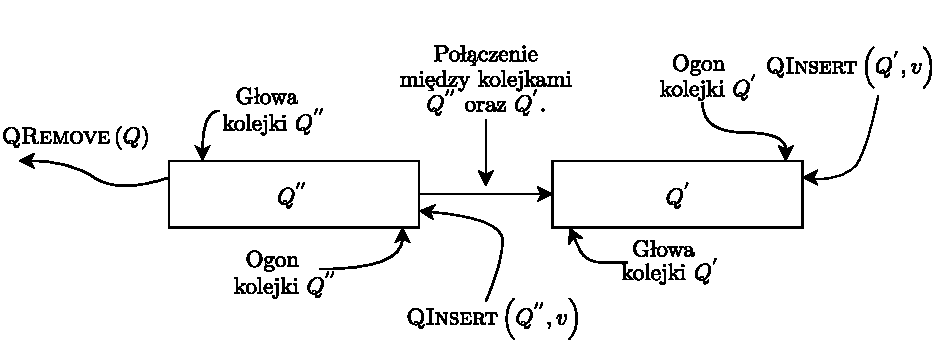
\includegraphics[width=\textwidth]{Chapter_III/GRAPH-GROWTH-2Q-Other/a.pdf}
	\caption{\textbf{Struktura wykorzystywana w~algorytmie $TQQ$} } \label{fig:exampleTQQStructure}
\end{figure}

Widzimy, że jedyna modyfikacja, jaka została dokonana w~oryginalnej strukturze, to przedefiniowanie operacji wstawiania elementów do struktury, która teraz wygląda w~następujący sposób:

\begin{itemize}
\item $\textrm{\textsc{QInsert}} \left( ?, v \right)$ --- gdy wierzchołka $v$ nie ma w~żadnej z~kolejek $Q^{'}$ i~$Q^{''}$ , w~zależności od właściwości danego wierzchołka wykonujemy jedną z~możliwych operacji:
\begin{itemize}
\item $\textrm{\textsc{QInsert}} \left( S, v \right) $ --- jeżeli wierzchołek, w~momencie wstawiania, jest osiągalny ze źródła ($v.d < \infty$) to jest on wstawiany na koniec kolejki $Q^{''}$,
\end{itemize}
\end{itemize}

Reszta operacji nie ulega zmianie, zaś analiza złożoności obliczeniowej pozostaje dokładnie taka sama (z wyjątkiem mniej kosztownej operacji wyszukiwania minimum w~kolejce priorytetowej)\footnote{Znowu możemy zrezygnować z własności kolejki priorytetowej i otrzymać złożoność na poziomie $O \left( n^{2} \cdot m \right)$. Może się jednak okazać, że dla pewnych grafów algorytm będzie dawał dość dobre wyniki~\cite[$3.10.2$]{Dissertation})}.

\begin{figure}[!htbp]
	\centering
	\begin{subfigure}[b]{0.28\textwidth}
		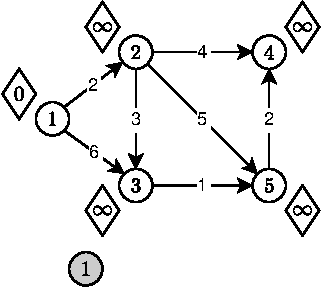
\includegraphics[width=\textwidth]{Chapter_III/GRAPH-GROWTH-2Q-Example/a.pdf}
		\caption{}
	\end{subfigure}
	\quad
	\begin{subfigure}[b]{0.28\textwidth}
		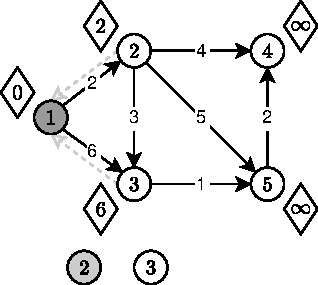
\includegraphics[width=\textwidth]{Chapter_III/GRAPH-GROWTH-2Q-Example/b.pdf}
		\caption{}
	\end{subfigure}
	\quad
	\begin{subfigure}[b]{0.28\textwidth}
		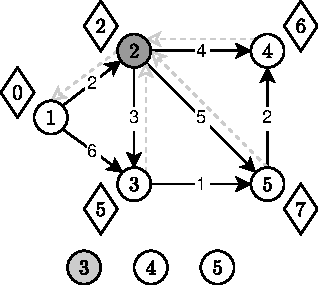
\includegraphics[width=\textwidth]{Chapter_III/GRAPH-GROWTH-2Q-Example/c.pdf}
		\caption{}
	\end{subfigure}
	\caption{\textbf{Działanie algorytmu z~dwoma kolejkami} \textbf{(a)} Algorytm rozpoczyna pracę ze źródłem w~wierzchołku $v_{1}$. \textbf{(b)} W~wyniku relaksacji jego krawędzi wychodzących na koniec kolejki $Q^{''}$ kolejno trafiają wierzchołki $v_{2}$ i~$v_{3}$. \textbf{(c)} Algorytm pobiera element ze stosu, wykonując dla krawędzi $e_{23}$, $e_{24}$, $e_{25}$ operację \textsc{RELAX}. } \label{fig:exampleDQQ1}
\end{figure}

\begin{figure}[!htbp]
	\ContinuedFloat
	\centering
	\begin{subfigure}[b]{0.28\textwidth}
		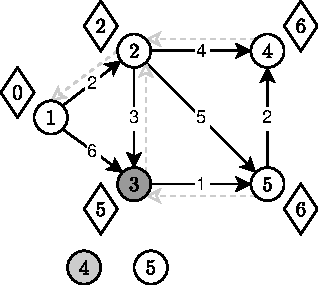
\includegraphics[width=\textwidth]{Chapter_III/GRAPH-GROWTH-2Q-Example/d.pdf}
		\caption{}
	\end{subfigure}
	\qquad	\qquad
	\begin{subfigure}[b]{0.28\textwidth}
		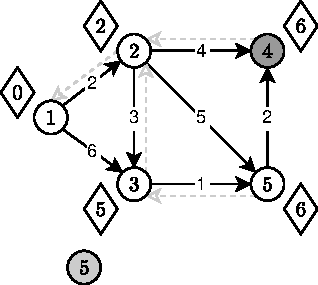
\includegraphics[width=\textwidth]{Chapter_III/GRAPH-GROWTH-2Q-Example/e.pdf}
		\caption{}
	\end{subfigure}
	\caption{ \textbf{(d--e)} Algorytm kontynuuje działanie według tego samego schematu, kończąc pracę w~momencie, gdy na żadnej z~kolejek $Q^{''}$ i~$Q^{'}$ nie ma już elementów. } \label{fig:exampleDQQ2}
\end{figure}


\section{Algorytm progowy}

Ostatnim algorytmem, jaki omówimy, będzie algorytm progowy (ang. \textit{Threshold algorithm}). Pojęcie progu pojawia się w~wielu dziedzinach informatyki (na przykład w~grafice komputerowej), oznaczając graniczną wartość, tyczącą się konkretnego zbioru danych, dla którego będącego poniżej/powyżej wartości progowej, ma zajść konkretna operacja. Nie inaczej jest w~przypadku algorytmu wyszukiwania najkrótszych ścieżek. Wartością progową tutaj, jak można się domyślić, będzie odległość wierzchołków od źródła w~czasie pracy algorytmu. Wszystkie krawędzie, których odległość będzie większa od zadanej wartości progowej, będą trafiały do zbioru wierzchołków, których badaniem zajmiemy się dopiero wówczas, gdy wykonamy wszystkie możliwe operacje dla pozostałych elementów. Gdy taka sytuacja nastąpi, wartość graniczna ulegnie stosownemu zwiększeniu, tym samym odległość pewnej liczby wierzchołków od źródła stanie się mniejsza niż nowo ustalony próg. Następnie algorytm wykona te same operacje, które wykonał dla wcześniejszego zbioru, kończąc dopiero pracę, gdy podniesie wartość progową na tyle wysoko, by zbiór wierzchołków, których odległość od źródła przekracza tą wartość, był pusty, podobnie jak zbiór pozostałych wierzchołków.

\begin{pseudokod}[!htbp]
\DontPrintSemicolon
\Begin{
	$ \textrm{\textsc{INIT-GRAPH}} \left( G, s \right)$ \;
	$ t \longleftarrow \textrm{wylicz wartość progową}$ \;
	$ L \longleftarrow \left\{ s \right\}$ \tcc*[f]{Lista, zawierająca wierzchołki $v : v.d < t$}\;
	$ \overline{L} \longleftarrow \emptyset $ \tcc*[f]{Lista, zawierająca pozostałe wierzchołki} \;
	\While(\tcc*[f]{Jeśli lista $\overline{L}$ była pusta to $L$ też jest.}){Lista $L$ nie pusta} {
		\While(\tcc*[f]{Opróżniamy listę $L$}){Lista $L$ nie pusta} {
			Usuń wierzchołek $v_{i}$ z~końca listy $ L $ \;
			\ForEach{$e_{ij} : v_{i} \overset{1} \leadsto v_{j}$}{
				$RELAX \left( v_{i}, v_{j} \right)$ \;
				\uIf{$ v_{j} \notin \left\{ L, \overline{L} \right\} $}{
					Wstaw węzeł $v_{j}$ na koniec $L$, jeśli $v_{j}.d < t$. W~przeciwnym przypadku wstaw na koniec $\overline{L}$ \;
				} \ElseIf{Po relaksacji $v_{j}.d < t$ i~$v_{j} \in \overline{L}$}{
					Przenieś węzeł $v_{j}$ na koniec listy $L$ \;
				}
			}
			$ t \longleftarrow t + \min \left\{ v.d : v \in \overline{L} \right\}$ \;
			Przepnij wszystkie $v : v.d < t $ do $L$ \;
		}
	}
}
\caption{ THR $\left( G, s \right)$\label{alg:ThresholdAlgorith}}
\end{pseudokod}

\subsubsection{Złożoność obliczeniowa}

W najgorszym możliwym przypadku wartość progowa na samym początku zostanie ustawiona na tyle wysoko, by wszystkie wierzchołki trafiły do listy $L$ (patrz \ref{alg:ThresholdAlgorith}). W~takim przypadku otrzymujemy natychmiastowo złożoność $O \left( m \cdot n \right)$, gdyż nie jesteśmy w~stanie nic powiedzieć o~kolejności skanowania wierzchołków (za każdym razem wybieramy po prostu ostatni z~listy, gdzie $ \left| L \right| = n $). Załóżmy jednak, że mamy daną wartość progową $t$ i~niech funkcja $L \left( i \right)$ oznacza zbiór wierzchołków, jakie znajdują się na liście $L$ po $i$'tym zwiększeniu wartości progowej.

\begin{itemize}
\item W~najgorszym możliwym przypadku największą odległością węzła od źródła będzie $ \left( n - 1 \right) \cdot C $. Znając wartość progową $t$ oraz zakładając, że za każdym razem w~zbiorze wierzchołków $\overline{L}$ najmniejszy wierzchołek $v_{min}$ to taki, dla którego $v_{min}.d = t + 1$, możemy wyznaczyć liczbę iteracji, jaką w~takim przypadku będzie musiał wykonać algorytm, nim skończy działanie. Takich iteracji zostanie wykonanych co najwyżej $ O \left( \frac{n \cdot C}{t}\right)$ (podobną analizę przeprowadziliśmy dla algorytmu, wykorzystującego kubełki z~przepełnieniem, gdzie ostatni kubełek można porównać do zbioru $\overline{L}$).
\item W~każdej $i$'tej iteracji do listy $L$ w~danym przypadku trafia $\left| L \left( i \right) \right|$ węzłów. Dla każdego z~nich zachodzi $t_{nowe} < v.d < t_{nowe} + t$. Wiedząc, że $t_{nowe} = \min \left\{ v.d : v \in \overline{L} \right\}$, możemy oszacować maksymalną liczbę razy, jaką każdy wierzchołek $v$ będzie skanowany, zanim nie zostanie usunięty z~aktualnej listy $L$. Ponownie wykorzystując analogię do analizy algorytmu kubełkowego (tym razem $DKA$), zauważmy, że z~każdą wykonaną relaksacją krawędzi, która prowadzi do wierzchołka $v$, jego odległość od źródła ulega zmniejszeniu o~co najmniej $1$. Zatem, jeżeli dla aktualnie badanego $L$ znajdują się w~nim wierzchołki, spełniające $t_{nowe} < v.d < t_{nowe} + t $, to po najwyżej $t$ skanowaniach wierzchołka $v$ zostanie on trwale usunięty z~listy $L$ (w następnych iteracjach do listy $L$ będą trafiać wierzchołki $u$ o~$u.d > v.d$, więc ponowna relaksacja krawędzi, wchodzącej do węzła $v$ na pewno nie zajdzie). Zatem nasz algorytm wykona maksymalnie $ O \left( m \cdot t \right)$ relaksacji.
\item W~każdej iteracji usunięcie wszystkich elementów z~$L \left( i~\right)$ zajmuje $ O \left( L \left( i~\right) \right)$. Z~faktu, że możemy wykonać maksymalnie $O \left( m \cdot t \right)$ relaksacji wynika, że podczas trwania algorytmu usuniemy co najwyżej $O \left( n \cdot t \right)$ wierzchołków.
\end{itemize}

Łącznie zatem otrzymujemy złożoność na poziomie $ O \left( m \cdot t + n \cdot t + \frac{n \cdot C}{t} \right) = O \left( m \cdot t + n \cdot \left( t + \frac{C}{t}\right) \right)$.

Niestety nie jest to koniec, przeprowadzanej przez nas analizy, gdyż ominęliśmy analizę czasu, jaki potrzebny jest do odnalezienia minimalnych wierzchołków w~$\overline{L}$ dla każdej z~$ O \left( \frac{n \cdot C}{t}\right)$ iteracji. Zakładając najgorszy możliwy przypadek, natychmiast otrzymujemy górne ograniczenie $O \left( n \cdot \frac{n \cdot C}{t} \right)$. Jest ono jednak bardzo niedokładne, gdyż zakłada, że z~każdą iteracją musimy przeszukać $O \left( n \right)$ wierzchołków w~$\overline{L}$, by znaleźć ten najmniejszy. Nie jest to prawdą, chociażby z~tego względu, że algorytm kończy działanie tylko wtedy, gdy w~powyższym zbiorze nie ma już żadnych elementów. Przyjmijmy zatem bardziej optymistyczną wersję: niech w~każdej z~$ O \left( \frac{n \cdot C}{t}\right)$ iteracji ze zbioru $\overline{L}$ będzie usuwanych tyle samo elementów. Daje nam to od razu ich liczbę: mamy $n-1$ wierzchołków, z~czego ich liczba w~liniowy sposób maleje w~czasie trwania wymienionej liczby iteracji a~zatem każdorazowo usuwanych jest ich $\frac{t}{C}$. W~czasie działania całego algorytmu suma liczby elementów w~zbiorze $\overline{L}$ wynosi zatem: 

\begin{equation}
	\begin{aligned}
		D &= \sum_{i=\frac{ \left( n-1 \right) \cdot C}{t}}^{1} i~\cdot \frac{t}{C} \approx \frac{t}{C} \cdot \sum_{i=1}^{\frac{n \cdot C}{t}} i\\
		&= \frac{t}{C} \cdot \frac{C \cdot n \cdot \left( C \cdot n + t \right)}{2 \cdot t^{2}} \\
		&= \frac{n \cdot \left( n \cdot C + t \right)}{2 \cdot t}.
	\end{aligned}
\end{equation}

Czas wyszukiwania minimalnego wierzchołka w~zbiorze $\overline{L}$ zawsze jest proporcjonalny do liczby jego elementów, więc ostatecznie mamy: $ O \left( \frac{n^{2} \cdot C}{t}\right)$. Taki sam wynik otrzymaliśmy dla analizy wcześniejszego przypadku. Tym samym złożoność całego algorytmu to $ O \left( m \cdot t + \frac{n^{2} \cdot C}{t}\right)$.

\begin{figure}[!h]
	\centering
	\begin{subfigure}[b]{0.32\textwidth}
		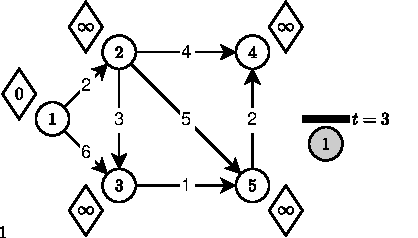
\includegraphics[width=\textwidth]{Chapter_III/THRESHOLD-Example/a.pdf}
		\caption{}
	\end{subfigure}
	\begin{subfigure}[b]{0.32\textwidth}
		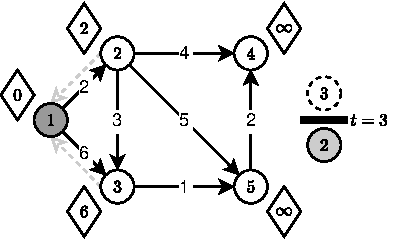
\includegraphics[width=\textwidth]{Chapter_III/THRESHOLD-Example/b.pdf}
		\caption{}
	\end{subfigure}
	\begin{subfigure}[b]{0.32\textwidth}
		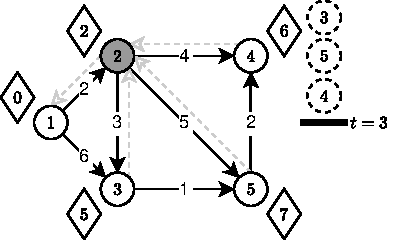
\includegraphics[width=\textwidth]{Chapter_III/THRESHOLD-Example/c.pdf}
		\caption{}
	\end{subfigure}
	\begin{subfigure}[b]{0.32\textwidth}
		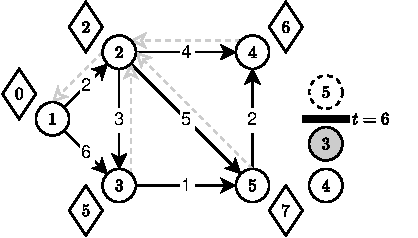
\includegraphics[width=\textwidth]{Chapter_III/THRESHOLD-Example/d.pdf}
		\caption{}
	\end{subfigure}
	\begin{subfigure}[b]{0.32\textwidth}
		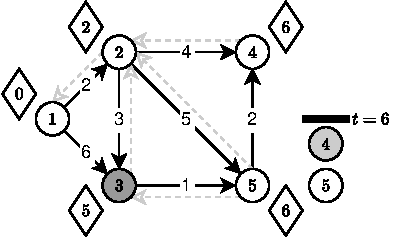
\includegraphics[width=\textwidth]{Chapter_III/THRESHOLD-Example/e.pdf}
		\caption{}
	\end{subfigure}
	\begin{subfigure}[b]{0.32\textwidth}
		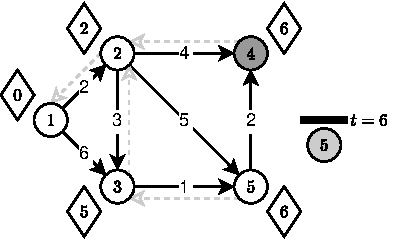
\includegraphics[width=\textwidth]{Chapter_III/THRESHOLD-Example/f.pdf}
		\caption{}
	\end{subfigure}
	\caption{ \textbf{(Działanie algorytmu opartego o~wartość progową} \textbf{(a)} Sytuacja po zainicjowaniu grafu $G = \left( V, E \right)$ przez \textsf{INIT-GRAPH} ($t=3$). Poniżej wartości progowej znajduje się węzeł $v_{1}$, będący źródłem. Powyżej znajduje się zawartość list $\overline{L}$ (obecnie pusta). \textbf{(b)} Sytuacja po wykonaniu relaksacji krawędzi $e_{12}$ oraz $e_{13}$. Wartość $v_{3}.d \geqslant t$ --- wierzchołek został wstawiony do $\overline{L}$. \textbf{(c)} Po wykonaniu relaksacji krawędzi wychodzących z~wierzchołka $v_{2}$, na koniec kolejki, ponad wartością progową, kolejno zostały dodane węzły: $v_{5}$ i~$v_{4}$. Lista $L$ jest pusta. \textbf{(d)} Próg zostaje zwiększony o~$t$ oraz zostały przeniesione na koniec kolejki wszystkie wierzchołki $v$, dla których $v.d < t$ (wierzchołki z~$\overline{L}$ do $L$ są przepinane w~kolejności od głowy pierwszej listy do ogona a~każdy węzeł zostaje wstawiony na koniec drugiego zbioru). \textbf{(e)} Z~listy $L$ zostaje pobrany minimalny wierzchołek a~następnie algorytm wykonuje relaksację krawędzi wychodzącej z~danego wierzchołka ($e_{35}$), w~wyniku czego węzeł $v_{5}$ zostaje przepięty na koniec listy $L$. \textbf{(f)} Po wykonaniu pozostałych relaksacji i~opróżnieniu listy $\overline{L}$ algorytm kończy działanie. } \label{fig:exampleThreshold}
\end{figure}

W naszym przypadku za wartość progową uznaliśmy średnią arytmetyczną kosztów wszystkich ścieżek w grafie, odpowiednio przemnożoną przez stałą, wyznaczaną przez ogólną gęstość grafu. Dokładniej:

\begin{eqnarray}
treshold = t \cdot \frac{PARAM}{DENCE}\textrm{,}
\end{eqnarray}
gdzie

\begin{eqnarray}
DENCE = \min \left( d, \frac{m}{n}\right) \\
t = \frac{1}{m} \cdot \sum_{e_{ij} \in E} c_{ij} \\
5 \leqslant PARAM \leqslant 10\textrm{.}
\end{eqnarray}

Przykład tak wybranego parametru algorytmu progowego można znaleźć w pracy Warrena Powella~\cite[$2$]{Threshold}.